\chapter{Utilizzo}

\section{Come trainer CW}
\`E possibile utilizzare lo Spider Keyer semplicemente collegando il paddle al jack stereo (potrebbe essere necessario usare un riduttore da 6.35 mm a 3.5 mm) e un caricabatterie al connettore mini USB.
In questa modalit\`a di funzionamento \`e sufficiente ruotare il potenziometro per modificare la velocit\`a tra un minimo di 15 WPM e un massimo di 40 WPM.

In questa modalit\`a non \`e possibile modificare ulteriori parametri (come il weighting o la modalit\`a iambic).

\section{Come keyer per pilotare la radio}
\begin{center}
	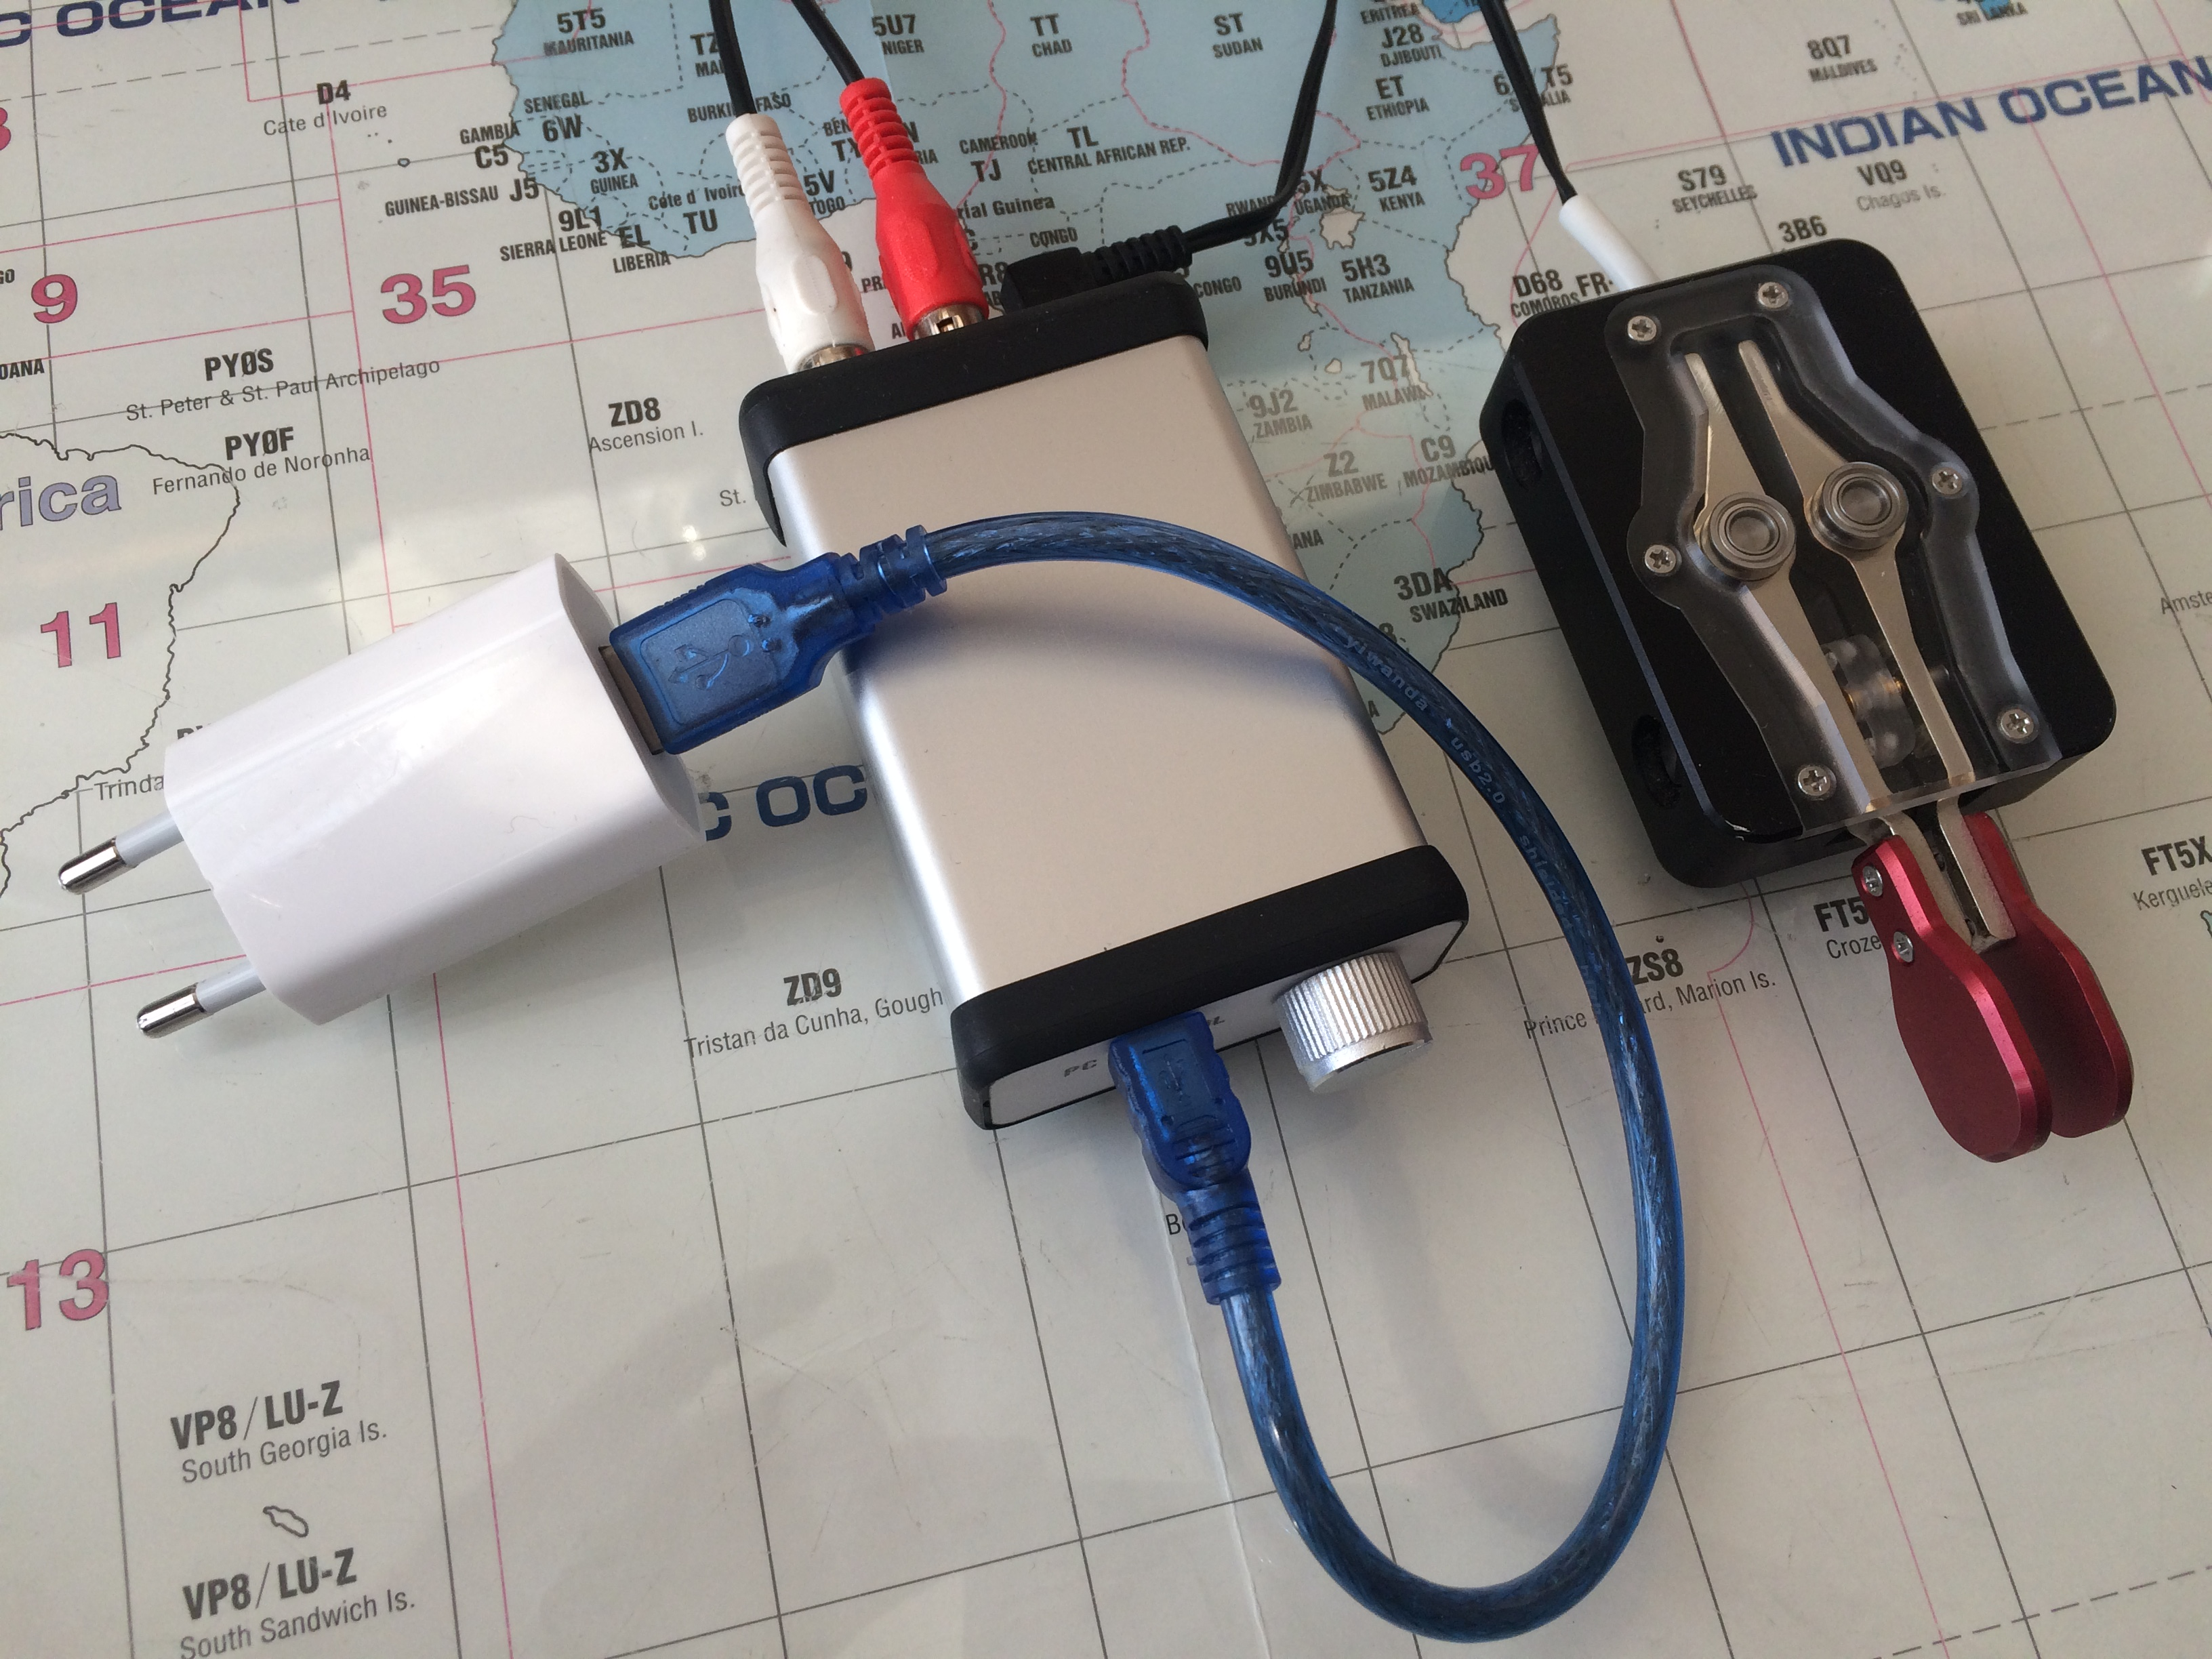
\includegraphics[width=\linewidth]{./Standalone.JPG}
\end{center}
Collegando l'uscita coassiale KEY (oltre al paddle e l'alimentazione USB), \`e possibile utilizzare una radio che non \`e dotata di keyer integrato (progettata per utilizare solo un tasto meccanico).

Collegando anche l'uscita coassiale PTT \`e possibile inoltre usare una radio che non \`e predisposta affatto per la trasmissione in CW.


\section{Insieme al software Ham Racer}
\begin{center}
	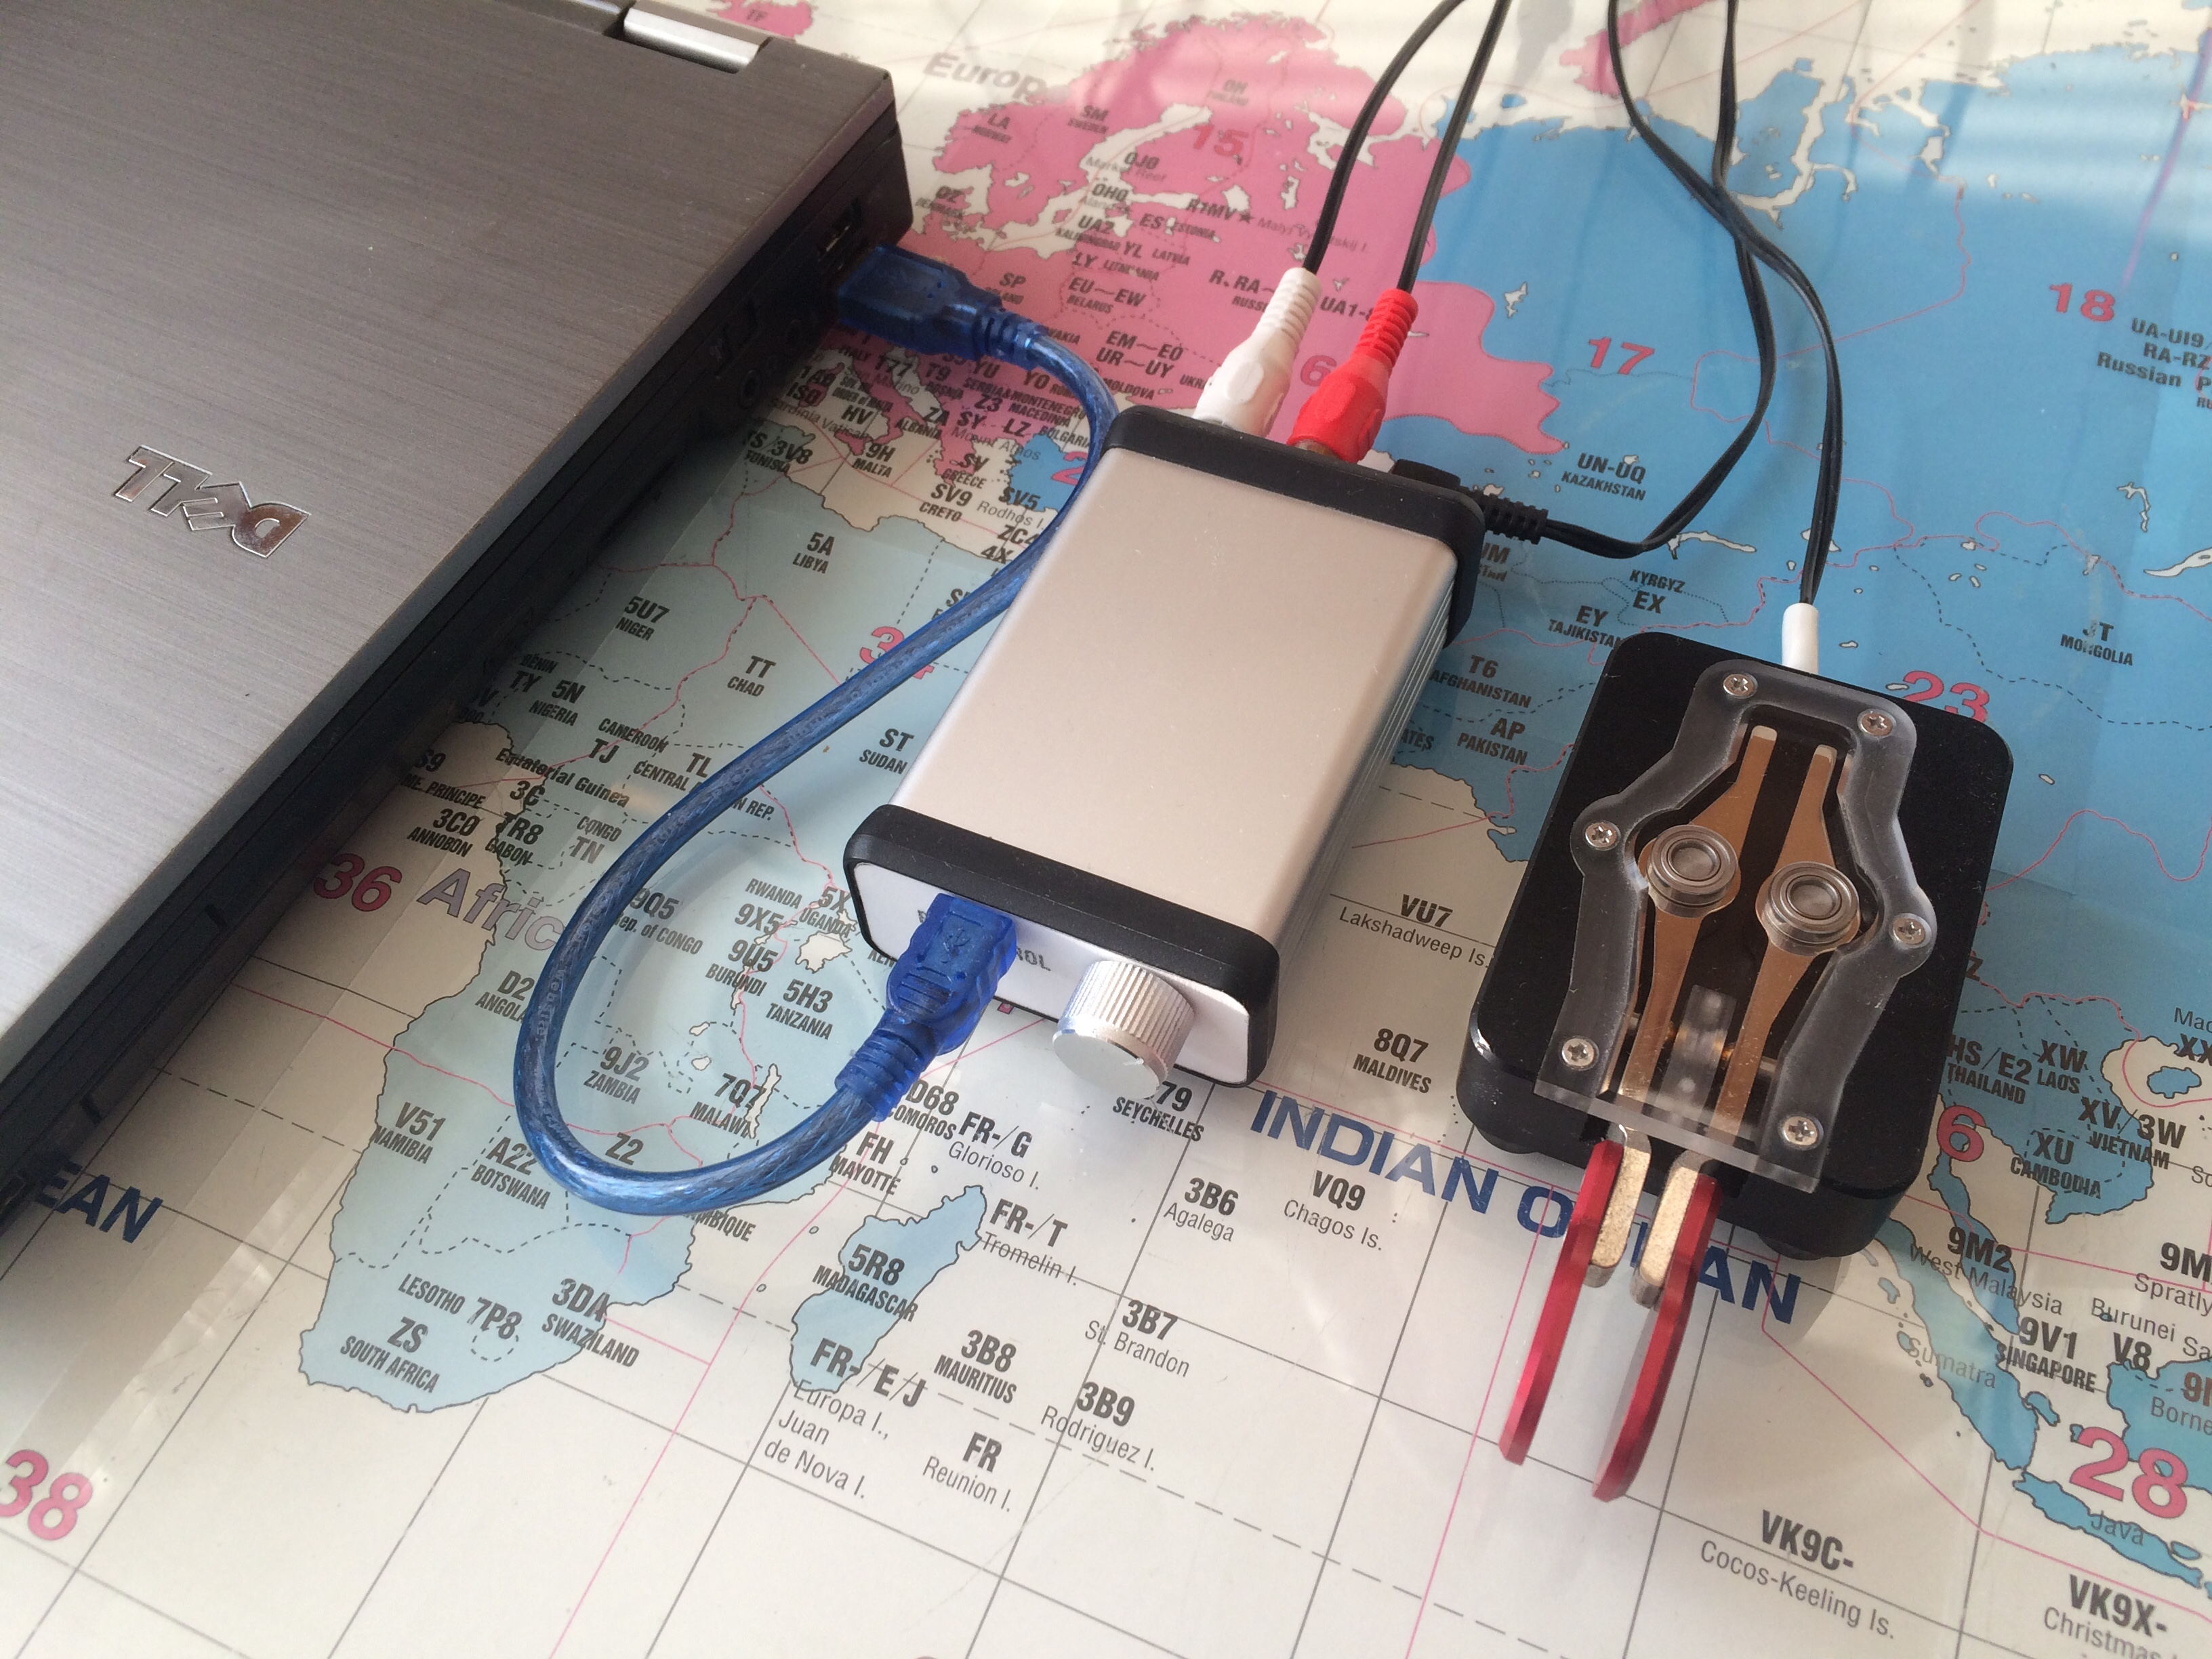
\includegraphics[width=\linewidth]{./PC.JPG}
\end{center}
Utilizzando un cavo USB (anzich\'e di alimentazione) e collegando lo Spider Keyer al PC, \`e possibile utilizzarlo all'interno del software Ham Racer (\url{http://ok1fig.nagano.cz/HamRacer/HamRacer.htm}), prodotto anch'esso da OK1FIG.

Ham Racer \`e un software progettato per i contest in SSB e CW e permette di realizzare QSO molto velocemente e di registrarli nel log integrato.
Poich\'e \`e impossibile parlare di tutte le funzionalit\`a che mette a disposizione in questo piccolo manuale, di seguito verranno descritte solo quelle inerenti all'utilizzo dello Spider Keyer.

\subsection{Connessione dello Spider Keyer ad Ham Racer}
Prima di poter utilizzare lo Spider Keyer \`e necessario connetterlo ad Ham Racer.
Questa operazione pu\`o essere effettuata una volta sola perch\'e Ham Racer \`e in grado di memorizzare a quale porta USB \`e stato collegato lo Spider Keyer e pu\`o quindi riconnettersi automaticamente.
\pagebreak
\begin{enumerate}
	\item Una volta avviato Ham Racer, impostare la modalit\`a di contest a CW (\texttt{Mode > CW}):
	\begin{center}
		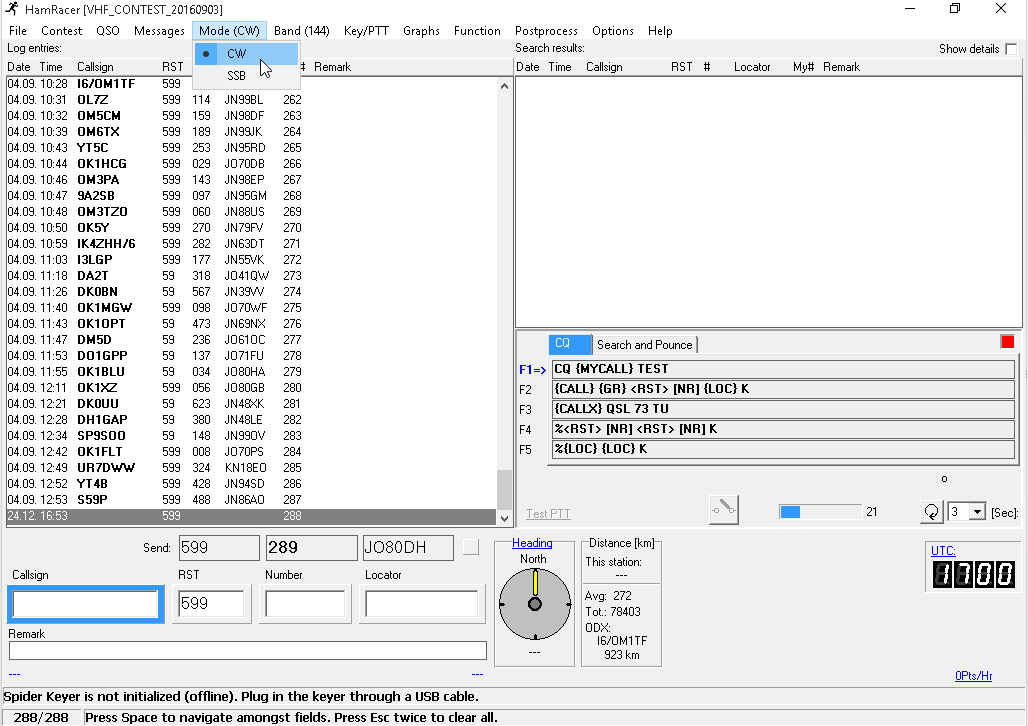
\includegraphics[width=\linewidth]{./hamracer01.png}
	\end{center}
	\item Fare click su \texttt{Key/PTT > Connect Device > Spider Keyer (Arduino Nano)}:
	\begin{center}
		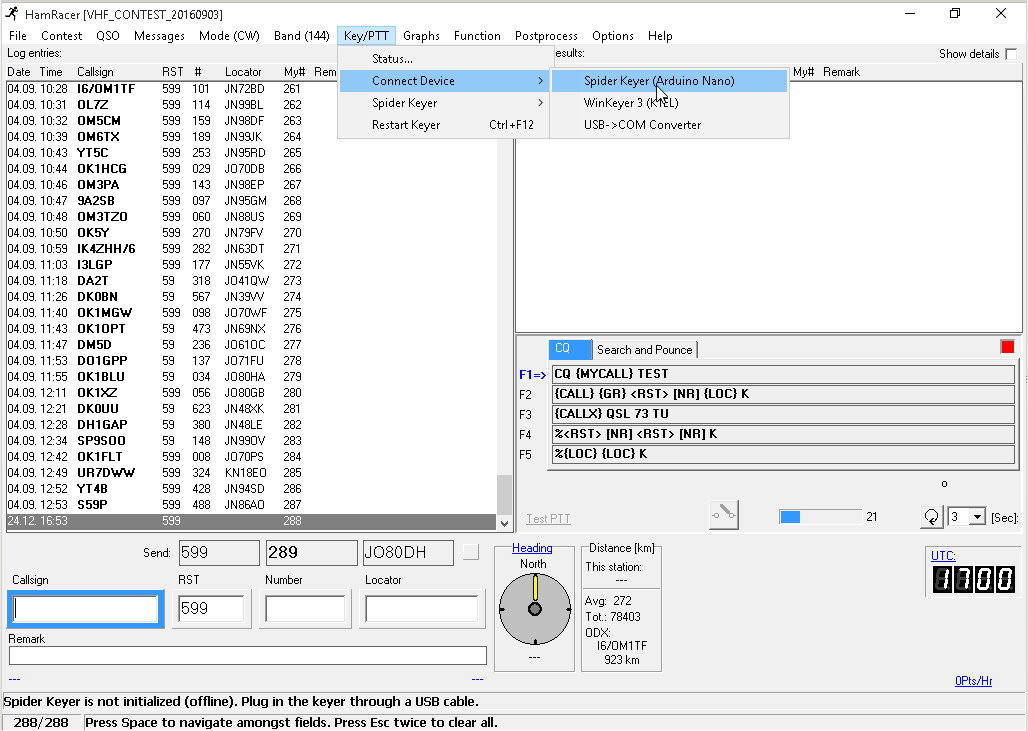
\includegraphics[width=\linewidth]{./hamracer02.png}
	\end{center}
\end{enumerate}
\pagebreak
\begin{enumerate}
		\item[3.] Disconnettere lo Spider Keyer dalla porta USB e fare click su \texttt{OK}:
	\begin{center}
		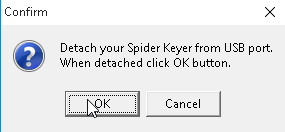
\includegraphics[width=\linewidth]{./hamracer03.png}
	\end{center}
		\item[4.] Dopo la fine della ricerca, ricollegare lo Spider Keyer alla porta USB e fare nuovamente click su \texttt{OK}:
	\begin{center}
		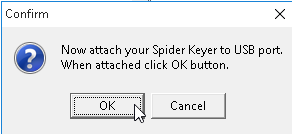
\includegraphics[width=\linewidth]{./hamracer04.png}
	\end{center}
\end{enumerate}
\begin{enumerate}
		\item[5.] Selezionare indifferentemente \texttt{Use the found COM port} o \texttt{Use the device's HW signature} e fare click su \texttt{OK}:
 	\begin{center}
		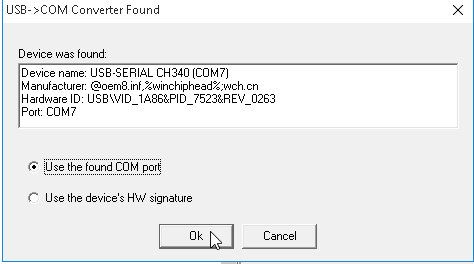
\includegraphics[width=\linewidth]{./hamracer05.png}
	\end{center}
		\item[6.] Lo Spider Keyer \`e ora connesso, ma per funzionare correttamente \`e consigliato disabilitare il VOX dalla radio:
	\begin{center}
		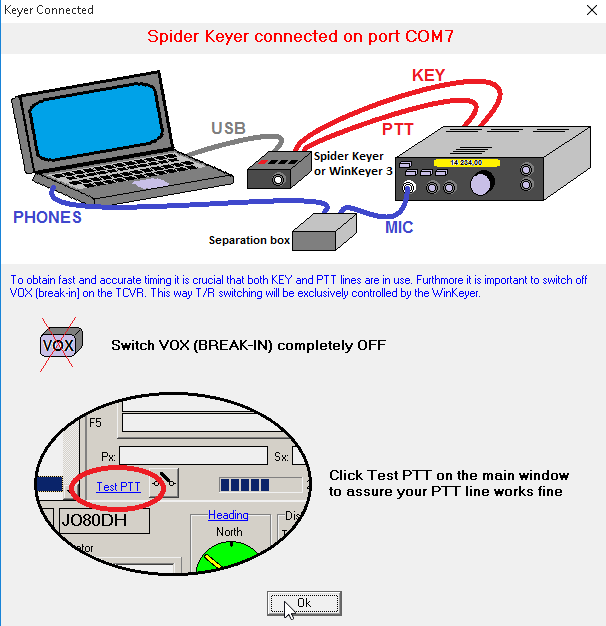
\includegraphics[width=\linewidth]{./hamracer06.png}
	\end{center}
\end{enumerate}
\pagebreak
\subsection{Configurazione dello Spider Keyer tramite Ham Racer}
	Dall'interfaccia principale di Ham Racer \`e possibile testare la corretta connessione tra Spider Keyer, PC e radio tramite il tasto \texttt{Test PTT}. Se tutto funziona correttamente, la radio andr\`a in trasmissione:
\begin{center}
	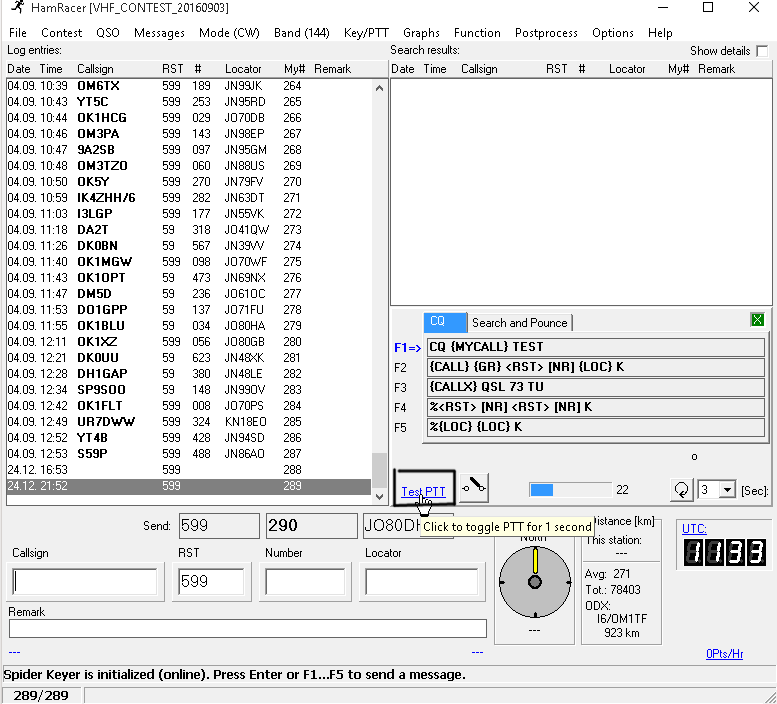
\includegraphics[width=\linewidth]{./config01.png}
\end{center}

\begin{samepage}
	Sempre dalla finestra principale, \`e possibile testare il cicalino, facendogli suonare un tono continuo con l'apposito tasto:
\begin{center}
	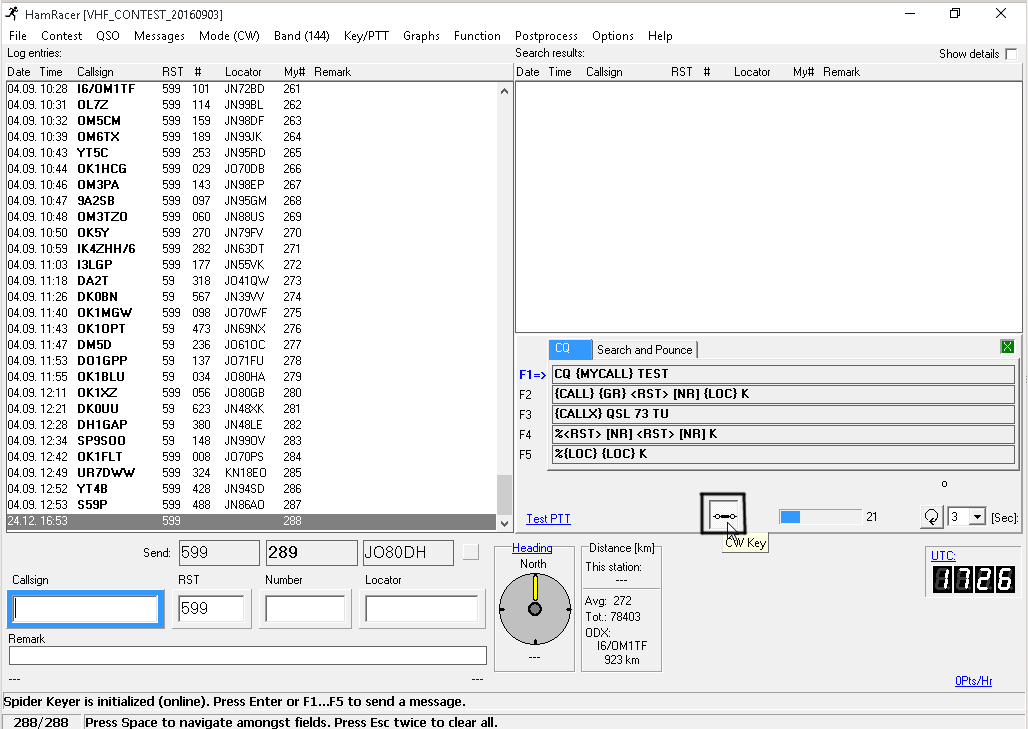
\includegraphics[width=\linewidth]{./config02.png}
\end{center}
\end{samepage}
\pagebreak
\begin{samepage}
	Il tasto di ripetizione permette di far ripetere a intervalli prefissati (ogni 3 secondi nella figura) i comandi inviati allo Spider Keyer:
	\begin{center}
	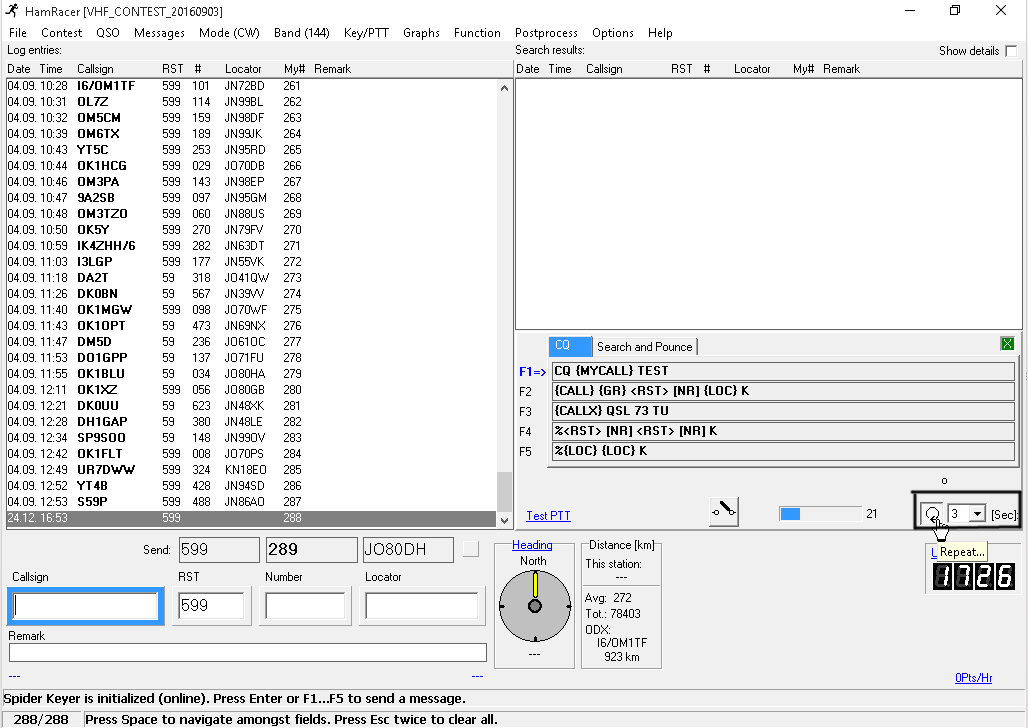
\includegraphics[width=\linewidth]{./config03.png}
\end{center}
\end{samepage}
\begin{samepage}
	\begin{center}
		La barra centrale mostra la velocit\`a attuale (in WPM), \`e possibile modificarla dal potenziometro oppure usando le frecce \texttt{su} e \texttt{gi\`u} della tastiera:
	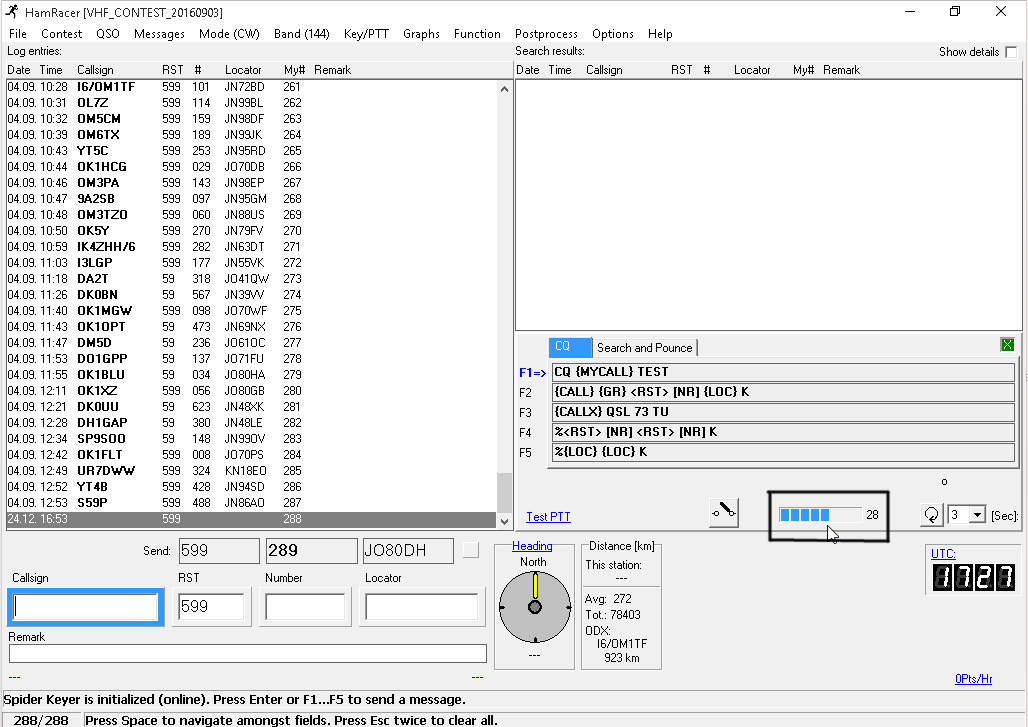
\includegraphics[width=\linewidth]{./config04.png}
\end{center}
\end{samepage}
\pagebreak
Per modificare le impostazioni avanzate del keyer:
\begin{enumerate}
	\item Fare click su \texttt{Options > Options}:
	\begin{center}
		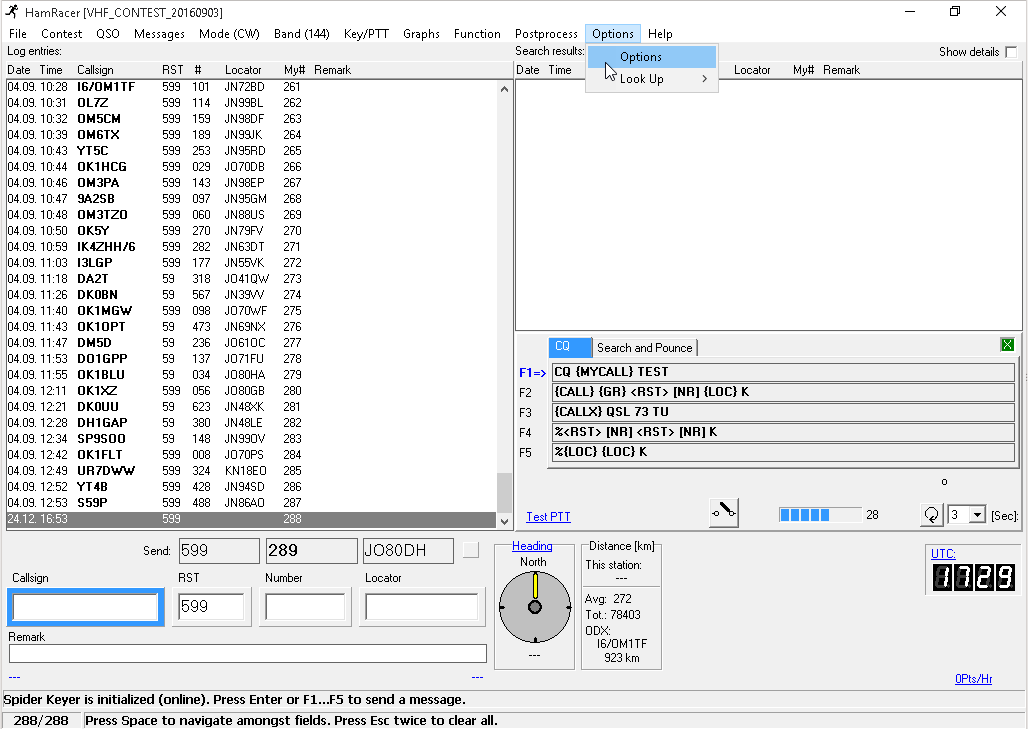
\includegraphics[width=\linewidth]{./config05.png}
	\end{center}
	\pagebreak
	\item Selezionare la linguetta \texttt{Spider Keyer} e modificare i ritardi del PTT all'inizio e alla fine della trasmissione:
	\begin{center}
		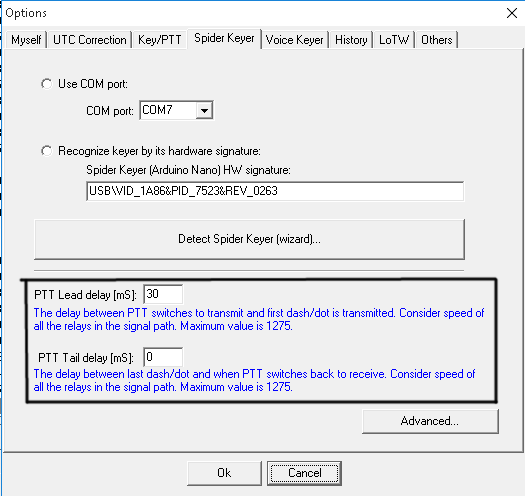
\includegraphics[width=\linewidth]{./config06.png}
	\end{center}
\pagebreak
	\item Fare click su \texttt{Advanced...} e settare le altre opzioni (frequenza del cicalino in trasmissione, sia in modalit\`a automatica che manuale, weighting, modalit\`a iambic, CW normalizzato e PTT attivato dalla trasmissione):
	\begin{center}
		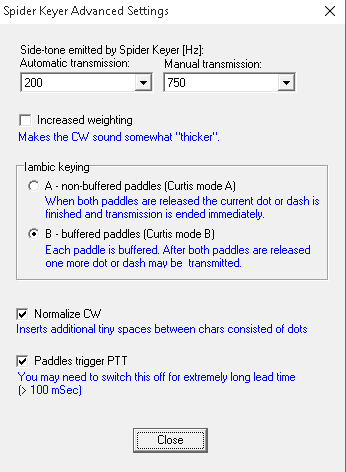
\includegraphics[width=\linewidth]{./config07.png}
	\end{center}
\end{enumerate}



\pagebreak
\subsection{Utilizzo dello Spider Keyer con Ham Racer}
Per qualunque necessit\`a, \`e possibile interrompere la trasmissione toccando il paddle, premendo il tasto \texttt{F12} o selezionando \texttt{Messages > Break Transmission} dal men\`u.

Ham Racer consente di inviare del testo qualsiasi (che verr\`a convertito automaticamente in dit e dah da trasmettere):
\begin{enumerate}
	\item Selezionare \texttt{Messages > Send Free Text} del men\`u:
	\begin{center}
		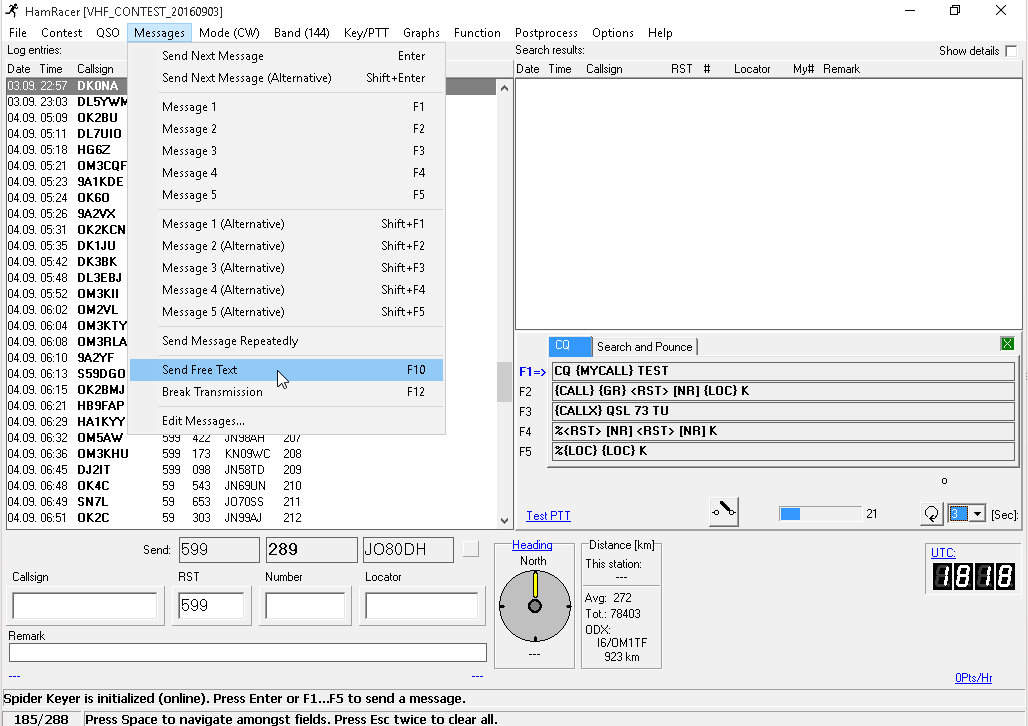
\includegraphics[width=\linewidth]{./use01.png}
	\end{center}
	\item Ad ogni \texttt{spazio} o \texttt{invio}, il testo viene trasmesso:
	\begin{center}
		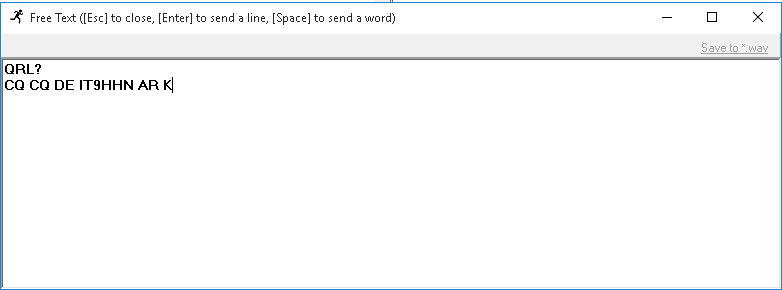
\includegraphics[width=\linewidth]{./use02.png}
	\end{center}
\end{enumerate}

Durante i contest \`e tuttavia preferibile avere messaggi gi\`a pronti da inviare velocemente. Ham Racer permette di configurare ben venti messaggi predefiniti per ognuna delle possibili combinazioni di contest (CW/SSB, HF/VHF/Expedition), ulteriormente suddivisi in messaggi di ricerca e messaggi di CQ.

\begin{samepage}
	Per trasmettere i messaggi predefiniti \`e sufficiente selezionare la linguetta corrispondente alla situazione desiderata (\texttt{CQ}/\texttt{Search and Pounce}) e premere i tasti da \texttt{F1} a \texttt{F5} per i primi cinque messaggi oppure \texttt{Maiusc} insieme ai tasti da \texttt{F1} a \texttt{F5} per gli altri cinque (in alternativa \`e possibile selezionarli con il mouse dal men\`u \texttt{Messages}):
\begin{center}
	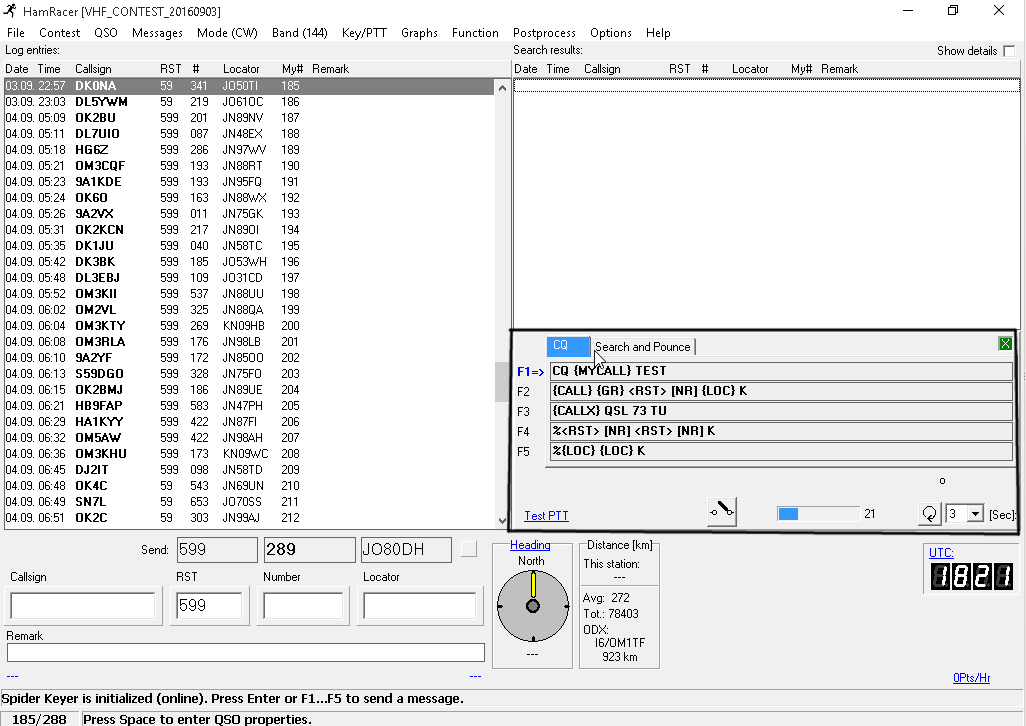
\includegraphics[width=\linewidth]{./use03.png}
\end{center}
\end{samepage}
\pagebreak
\`E inoltre possibile modificare i messaggi predefiniti:
\begin{enumerate}
	\item Fare click su \texttt{Messages > Edit Messages...}:
	\begin{center}
		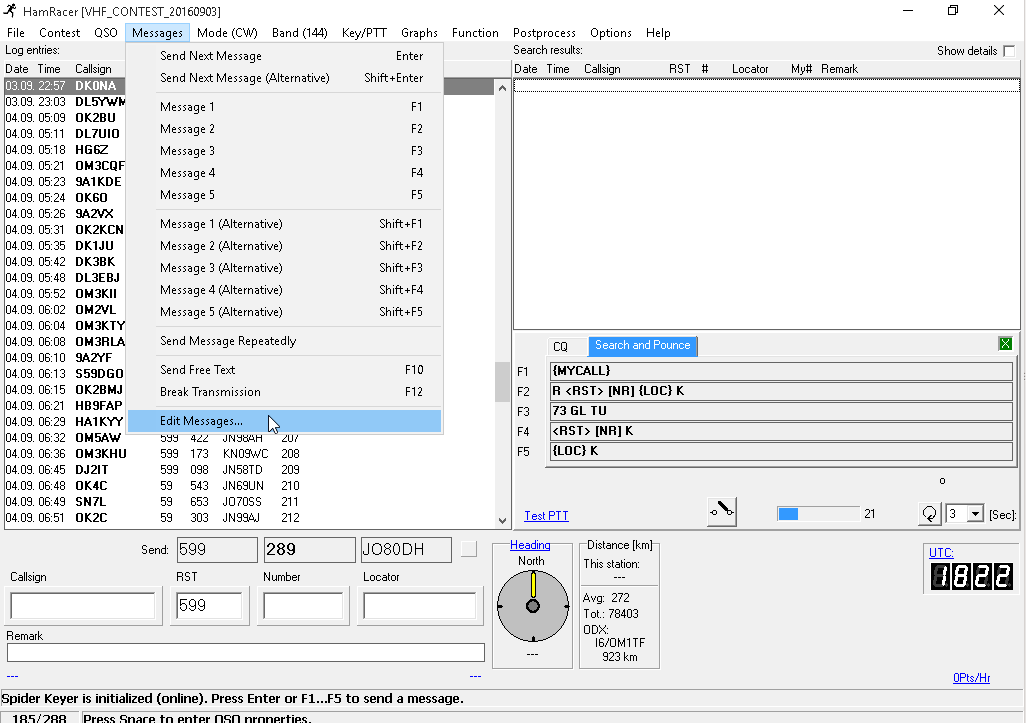
\includegraphics[width=\linewidth]{./use04.png}
	\end{center}
	\item Modificare i messaggi secondo le proprie esigenze, per ognuna delle modalit\`a di contest:
	\begin{center}
		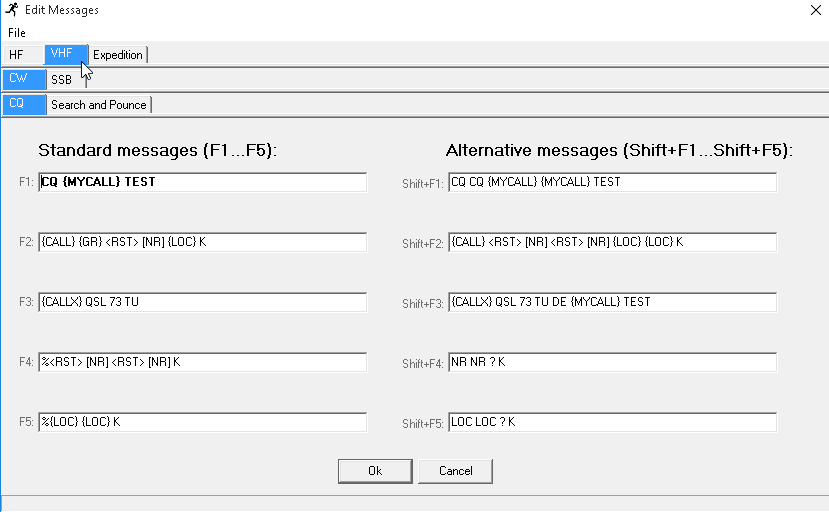
\includegraphics[width=\linewidth]{./use05.png}
	\end{center}
\end{enumerate}

All'interno dei messaggi predefiniti (non quelli mandati come testo libero) \`e possibile utilizzare dei segnaposto che verranno automaticamente sostituiti da Ham Racer (ad esempio il messaggio \texttt{\{CALLX\} QSL 73 TU} verr\`a trasmesso come \texttt{I6ORZ QSL 73 TU} se sul log si \`e registrato il QSO con I6ORZ).

\begin{table}[h]
	\begin{center}
		\rowcolors{2}{white}{gray!25}
		\begin{tabular}{ll}	
			\rowcolor{gray!50}
			Segnaposto & Significato\\
			\texttt{\{RS\}}& Rapporto RS da inviare\\
			\texttt{\{RST\}}& Rapporto RST da inviare\\			
			\texttt{\{NR\}}& Numero di QSO da inviare\\
			\texttt{\{LOC\}}& Locatore da inviare (solo per contest VHF)\\
			\texttt{\{CALL\}}& Nominativo ricevuto\\
			\texttt{\{CALLX\}}& Nominativo ricevuto dopo una correzione\\
			\texttt{\{MYCALL\}}& Nominativo da inviare\\
			\texttt{\{ABR\}}& Abbreviazione del nome del contest (solo per contest CW)\\
			\texttt{\{GR\}}& Saluto automatico (\texttt{GM} di giorno, \texttt{GA} di pomeriggio e \texttt{GE} di sera)\\
		\end{tabular}
	\end{center}
	\caption{Segnaposto interpretati da Ham Racer}
	\label{tab:plc}
\end{table}


I segnaposto racchiusi tra parentesi graffe sono trasmessi semplicemente sostituendo il valore, i segnaposto racchiusi tra parentesi quadre sostituiscono anche lo zero con una \texttt{T} (utili per trasmettere il numero di QSO) e quelli tra parentesi angolari sostituiscono lo zero con una \texttt{T} e il nove con una \texttt{N} (utile per gli RST).
Per esempio, volendo dare un RST di 590 (facendo finta che 0 sia un tono valido) si ottengono i seguenti risultati:
\begin{table}[h]
	\begin{center}
		\rowcolors{2}{white}{gray!25}
		\begin{tabular}{lll}	
			\rowcolor{gray!50}
			Segnaposto & Testo & CW\\
			\texttt{\{RST\}}& \texttt{590} & \texttt{..... ----. -----}\\
			\texttt{[RST]}& \texttt{59T} & \texttt{..... ----. -}\\
			\texttt{<RST>}& \texttt{5NT} & \texttt{..... -. -}\\
		\end{tabular}
	\end{center}
	\caption{Segnaposto RST = 590 interpretati da Ham Racer}
	\label{tab:rst}
\end{table}


\section{Comunicazione seriale avanzata}
\`E inoltre possibile comunicare con lo Spider Keyer tramite qualsiasi software di comunicazione seriale (ad esempio \url{putty.org}), settando:
\begin{itemize}
	\item Velocit\`a: \texttt{57600 baud};
	\item Bit dati: \texttt{8};
	\item Bit stop: \texttt{2};
	\item Parit\`a: \texttt{Nessuna};
	\item Controllo di flusso: \texttt{XON/XOFF}.
\end{itemize}

Ogni stringa costituita da caratteri stampabili che viene inviata allo Spider Keyer \`e convertita automaticamente in dit e dah che vengono suonati dal cicalino o inviati alla radio. Ad esempio, inviando via seriale il testo ``\texttt{CQ}'', il cicalino suoner\`a ``\texttt{-.-. -\--.-}''.

\begin{table}[h!]
	\begin{center}
		\rowcolors{2}{white}{gray!25}
		\begin{tabular}{llllllllll}		
			A&B&C&D&E&F&G&H&I&J\\
			K&L&M&N&O&P&Q&R&S&T\\
			U&V&W&X&Y&Z&&&&\\
			0&1&2&3&4&5&6&7&8&9\\
			=&/& &*&.&,&'&!&?&(\\
			)&\&&:&;&+&-&\_&"&\$&@\\
			$<$&$>$&&&&&&&&\\
			\end{tabular}
	\end{center}
	\caption{Caratteri riconosciuti dallo Spider Keyer (le lettere devono essere trasmesse in maiuscolo)}
	\label{tab:0}
\end{table}

Inviando lo spazio o un a capo (\texttt{\textbackslash r\textbackslash n}) comincia la trasmissione del messaggio, che pu\`o essere interrotta inviando un comando immediato (vedi sezione \ref{sec:cmds}) o premendo i tasti sul paddle.


Lo Spider Keyer rimane inoltre in ascolto per comandi costituiti da due byte (sezione \ref{sec:cmds}) e, dopo averli eseguiti, pu\`o rispondere con altri due byte (sezione \ref{sec:rps}) o una stringa identificativa (nel caso del comando \texttt{CMD\_GET\_SIGNATURE}).

\subsection{Comandi}\label{sec:cmds}
I comandi possono essere eseguiti in modalit\`a bufferizzata (prima finisce di fare quello che sta facendo, ad esempio la trasmissione di un segnale alla radio, e poi esegue il comando) o immediata.
Per eseguire i comandi in modalit\`a immediata, \`e necessario mandare prima del comando il byte \texttt{0x27 (ESC)}.


Il primo byte di ogni comando indica il tipo di operazione da eseguire e il secondo indica eventuali parametri.
Di seguito vengono elencati tutti i comandi (tra parentesi il valore del primo byte).

Nota bene: i nomi mnemonici sono indicati solo per una facile memorizzazione: i comandi sono inviati trasmettendo i bytes corrispondenti, non il nome mnemonico (ad esempio per far suonare il cicalino, bisogna trasmettere \texttt{0x12 0x00}, non \texttt{CMD\_BEEP}).

\subsubsection{\texttt{CMD\_SET\_PTT (0x01)}}
\begin{itemize}
	\item Effetto: Attiva/disattiva PTT
	\item Secondo byte:
	\begin{itemize}
		\item \texttt{0x00}: Disattiva il PTT
		\item \texttt{altro}: Attiva il PTT
	\end{itemize}
	\item Modalit\`a: Solo immediata.
\end{itemize}

\subsubsection{\texttt{CMD\_SET\_KEY (0x02)}}
\begin{itemize}
	\item Effetto: Attiva/disattiva la nota
	\item Secondo byte:
	\begin{itemize}
		\item \texttt{0x00}: Rilascia il tasto
		\item \texttt{0x01}: Preme il tasto, ma senza attivare il PTT
		\item \texttt{0x02}: Preme il tasto dopo aver attivato il PTT
	\end{itemize}
	\item Modalit\`a: Solo immediata.
\end{itemize}

\subsubsection{\texttt{CMD\_SPEED\_CHANGE (0x03)}}
\begin{itemize}
	\item Effetto: Setta la velocit\`a in WPM
	\item Secondo byte:
	\begin{itemize}
		\item \texttt{0x00}: Annulla un cambio di velocit\`a bufferizzato
		\item \texttt{0xFF}: Regola in base al potenziometro
		\item \texttt{tra 0x10 e 0x28}: Regola ai WPM corrispondenti (per esempio 0x1D = 29 WPM)
	\end{itemize}
	\item Valore predefinito: Regola in base al potenziometro
	\item Modalit\`a: Sia immediata che bufferizzata.
\end{itemize}

\subsubsection{\texttt{CMD\_SET\_LEAD\_TIME (0x04)}}
\begin{itemize}
	\item Effetto: Setta il tempo che intercorre tra l'attivazione del PTT e il primo simbolo trasmesso
	\item Secondo byte: Tempo in scatti da 5 ms (per esempio 0x10 = 16 $\rightarrow$ 80 ms)
	\item Valore predefinito: 30 ms
	\item Modalit\`a: Solo immediata.
\end{itemize}

\subsubsection{\texttt{CMD\_SET\_TAIL\_TIME (0x05)}}
\begin{itemize}
	\item Effetto: Setta il tempo in cui il PTT rimane attivo dopo l'ultimo simbolo trasmesso
	\item Secondo byte: Tempo in scatti da 5 ms (per esempio 0x3A = 58 $\rightarrow$ 290 ms)
	\item Valore predefinito: 5 ms
	\item Modalit\`a: Solo immediata.
\end{itemize}

\subsubsection{\texttt{CMD\_SET\_HANG\_TIME (0x06)}}
\begin{itemize}
	\item Effetto: Setta il tempo tra la fine della trasmissione e il passaggio in ricezione quando si usa il paddle
	\item Secondo byte: Tempo in percentuale di lunghezza di parola (PARIS)
	\item Valore predefinito: 90\%
	\item Modalit\`a: Solo immediata.
\end{itemize}

\subsubsection{\texttt{CMD\_SET\_WEIGHTING (0x07)}}
\begin{itemize}
	\item Effetto: Setta il weighting tra dit e dah
	\item Secondo byte: Percentuale di weighting
	\item Valore predefinito: 50\%
	\item Modalit\`a: Solo immediata.
\end{itemize}

\subsubsection{\texttt{CMD\_SET\_PADDLES\_TRIGGER\_PTT (0x09)}}
\begin{itemize}
	\item Effetto: Attiva/disattiva il PTT automatico con il paddle
	\item Secondo byte:
	\begin{itemize}
		\item \texttt{0x00}: PTT non attivato dal paddle
		\item \texttt{altro}: PTT attivato dal paddle
	\end{itemize}
	\item Valore predefinito: PTT attivato
	\item Modalit\`a: Solo immediata.
\end{itemize}

\subsubsection{\texttt{CMD\_SET\_SIDETONE\_AUTOMATIC (0x0A)}}
\begin{itemize}
	\item Effetto: Setta la frequenza del cicalino quando trasmette il segnale proveniente dal PC
	\item Secondo byte: Frequenza in scatti da 10 Hz (per esempio 0x5A = 90 $\rightarrow$ 900 Hz)
	\item Valore predefinito: 750 Hz
	\item Modalit\`a: Sia immediata che bufferizzabile.
\end{itemize}

\subsubsection{\texttt{CMD\_SET\_SIDETONE\_MANUAL (0x0B)}}
\begin{itemize}
	\item Effetto: Setta la frequenza del cicalino quando trasmette il segnale proveniente dal paddle
	\item Secondo byte: Frequenza in scatti da 10 Hz (per esempio 0x53 = 83 $\rightarrow$ 830 Hz)
	\item Valore predefinito: 750 Hz
	\item Modalit\`a: Solo immediata.
\end{itemize}

\subsubsection{\texttt{CMD\_SET\_IAMBIC\_MODE (0x0C)}}
\begin{itemize}
	\item Effetto: Setta modalit\`a di trasmissione iambic
	\item Secondo byte:
	\begin{itemize}
		\item \texttt{0x00}: Modalit\`a Curtis A
		\item \texttt{0x01}: Modalit\`a Curtis B
	\end{itemize}
	\item Valore predefinito: Curtis B
	\item Modalit\`a: Solo immediata.
\end{itemize}

\subsubsection{\texttt{CMD\_SET\_BREAK\_IMMY (0x0E)}}
\begin{itemize}
	\item Effetto: Interrompe immediatamente la trasmissione
	\item Secondo byte: qualsiasi
	\item Modalit\`a: Solo immediata.
\end{itemize}

\subsubsection{\texttt{CMD\_RESET (0x0F)}}
\begin{itemize}
	\item Effetto: Ripristina i valori predefiniti e resetta lo Spider Keyer
	\item Secondo byte: qualsiasi
	\item Modalit\`a: Solo immediata.
\end{itemize}

\subsubsection{\texttt{CMD\_PING (0x10)}}
\begin{itemize}
	\item Effetto: Invia due byte di risposta
	\item Secondo byte: qualsiasi
	\item Modalit\`a: Sia immediata che bufferizzabile.
\end{itemize}

\subsubsection{\texttt{CMD\_GET\_SIGNATURE (0x11)}}
\begin{itemize}
	\item Effetto: Invia la firma del dispositivo
	\item Secondo byte: qualsiasi
	\item Modalit\`a: Solo immediata.
\end{itemize}

\subsubsection{\texttt{CMD\_BEEP (0x12)}}
\begin{itemize}
	\item Effetto: Fa suonare il cicalino
	\item Secondo byte: qualsiasi
	\item Modalit\`a: Sia immediata che bufferizzabile.
\end{itemize}

\subsubsection{\texttt{CMD\_SET\_FEEDBACK (0x13)}}
\begin{itemize}
	\item Effetto: Attiva/disattiva la trasmissione automatica dei byte di risposta allo scatenarsi di eventi
	\item Secondo byte:
	\begin{itemize}
		\item \texttt{0x00}: Disattiva
		\item \texttt{altro}: Attiva
	\end{itemize}
	\item Valore predefinito: Disattiva
	\item Modalit\`a: Solo immediata.
\end{itemize}


\subsection{Risposte}\label{sec:rps}
Lo Spider Keyer invia al PC delle risposte allo scatenarsi di eventi:
\begin{itemize}
	\item \`E stato inviato il comando \texttt{CMD\_PING}
	\item \`E attivato il comando \texttt{CMD\_SET\_FEEDBACK} e succede qualcosa (come un cambio di velocit\`a dal potenziometro).
\end{itemize}

La risposta \`e costituita da due byte, il primo notifica lo stato attuale (tabella \ref{tab:1}), mentre il secondo la velocit\`a impostata (tabella \ref{tab:2}).

\begin{table}[h]
	\begin{center}
		\begin{tabular}{ll}
			\rowcolor{gray!50}
			Bit & Significato\\
			\rowcolor{white}
			7 (MSB) & sempre 1\\
			\rowcolor{gray!25}
			6 & non usato\\
			\rowcolor{white}
			\multirow{2}{*}{5} & 0: buffer vuoto\\
			& 1: caratteri disponibili nel buffer\\
			\rowcolor{gray!25}
			& 0: PTT spento\\
			\rowcolor{gray!25}
			\multirow{-2}{*}{4} & 1: PTT acceso\\
			\rowcolor{white}
			& 0: tasto off\\
			\rowcolor{white}
			& 1: tasto on\\
			\rowcolor{white}
			\multirow{-3}{*}{3} & NOTA: questo bit \`e settato solo da \texttt{CMD\_SET\_KEY}, non dal paddle\\
			\rowcolor{gray!25}
			2 & non usato\\
			\rowcolor{white}
			1 & non usato\\
			\rowcolor{gray!25}
			0 (LSB) & non usato\\
		\end{tabular}
	\end{center}
	\caption{Primo byte di risposta}
	\label{tab:1}
\end{table}

\begin{table}[h]
	\begin{center}
		\begin{tabular}{ll}
			\rowcolor{gray!50}
			Bit & Significato\\
			\rowcolor{white}
			7 (MSB) & sempre 0\\
			\rowcolor{gray!25}
			& 0: velocit\`a cambiata da \texttt{CMD\_SPEED\_CHANGE}\\
			\rowcolor{gray!25}
			\multirow{-2}{*}{6-0} & altro: nuova velocit\`a se impostata dal potenziometro\\
		\end{tabular}
	\end{center}
	\caption{Secondo byte di risposta}
	\label{tab:2}
\end{table}